
\documentclass[11pt,fleqn]{article} 
\usepackage[margin=0.8in, head=0.8in]{geometry} 
\usepackage{amsmath, amssymb, amsthm}
\usepackage{fancyhdr} 
\usepackage{palatino, url, multicol}
\usepackage{graphicx, pgfplots} 
\usepackage[all]{xy}
\usepackage{polynom} 
%\usepackage{pdfsync} %% I don't know why this messes up tabular column widths
\usepackage{enumerate}
\usepackage{framed}
\usepackage{setspace}
\usepackage{array,tikz}

\pgfplotsset{compat=1.6}

\pgfplotsset{soldot/.style={color=black,only marks,mark=*}} \pgfplotsset{holdot/.style={color=black,fill=white,only marks,mark=*}}


\pagestyle{fancy} 
\lfoot{}
\rfoot{\S 2.4}

\begin{document}
\renewcommand{\headrulewidth}{0pt}
\newcommand{\blank}[1]{\rule{#1}{0.75pt}}
\newcommand{\bc}{\begin{center}}
\newcommand{\ec}{\end{center}}
\renewcommand{\d}{\displaystyle}

\vspace*{-0.7in}

%%%%%%%%%intro page
\begin{center}
  \large
  \sc{Section 2.4: Arc Length of a Curve and Surface Area}\\
  day 2
 
\end{center}


\begin{quote}
Set up, \emph{but do not evaluate}, definite integrals for these length and area problems.
\end{quote}
\bigskip
\begin{enumerate}
\item  Find the length of the curve {\large $y=e^x$} from $x=0$ to $x=1$.
\vfill

\item   Find the surface area of the surface of revolution from rotating {\large $y=e^x$} from $x=0$ to $x=1$ around the $x$-axis.
\vfill

\item   Find the length of the curve {\large $y=\frac{x^4}{4}+\frac{1}{8x^2}$} from $x=1$ to $x=2$.
\vfill

\clearpage
\newpage
\item  Find the surface area of the surface of revolution from rotating {\large $y=x^2$} from $x=0$ to $x=1$ around the $y$-axis.
\vfill


\item   Find the length of the curve {\large $x^{2/3}+y^{2/3}=4$} (graphed below).\\
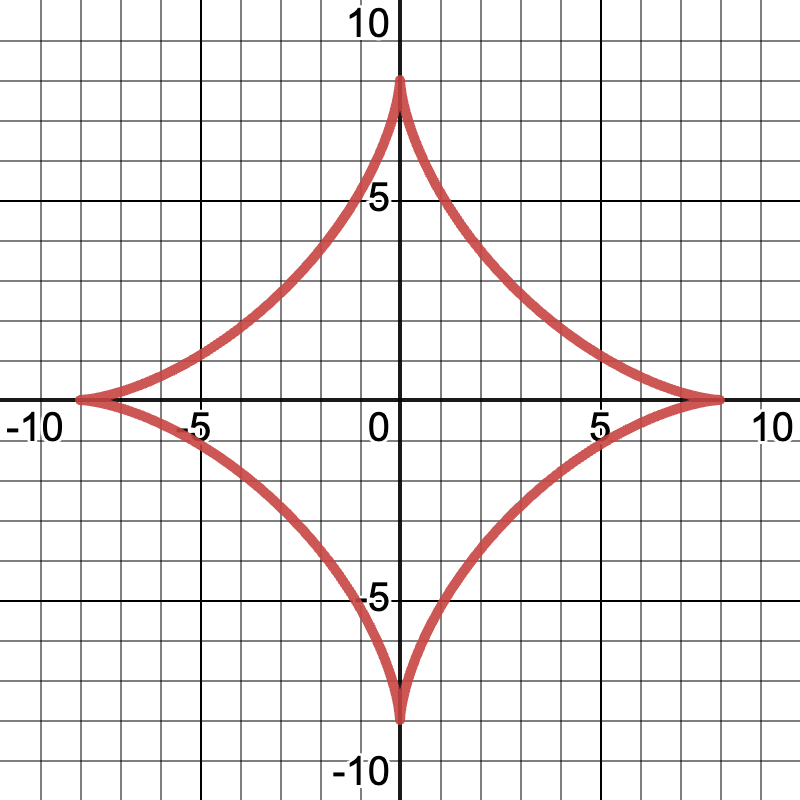
\includegraphics[scale=0.2]{pic-2-4-a.png}
\vfill


\item   Now do triage.  Which of the integrals in problems \textbf{1} through \textbf{5} can actually be computed by hand?  Try those.   For the others, go online and use your favorite tool to compute values for the definite integrals.
-
\end{enumerate}
\end{document}

